%%% lorem.tex --- 
%% 
%% Filename: lorem.tex
%% Description: 
%% Author: Ola Leifler
%% Maintainer: 
%% Created: Wed Nov 10 09:59:23 2010 (CET)
%% Version: $Id$
%% Version: 
%% Last-Updated: Wed Nov 10 09:59:47 2010 (CET)
%%           By: Ola Leifler
%%     Update #: 2
%% URL: 
%% Keywords: 
%% Compatibility: 
%% 
%%%%%%%%%%%%%%%%%%%%%%%%%%%%%%%%%%%%%%%%%%%%%%%%%%%%%%%%%%%%%%%%%%%%%%
%% 
%%% Commentary: 
%% 
%% 
%% 
%%%%%%%%%%%%%%%%%%%%%%%%%%%%%%%%%%%%%%%%%%%%%%%%%%%%%%%%%%%%%%%%%%%%%%
%% 
%%% Change log:
%% 
%% 
%% RCS $Log$
%%%%%%%%%%%%%%%%%%%%%%%%%%%%%%%%%%%%%%%%%%%%%%%%%%%%%%%%%%%%%%%%%%%%%%
%% 
%%% Code:

\chapter{Method}
\label{cha:method}
This chapter describes the proposed system for arrival time prediction
and event detection, and its implementation.

\section{System Description}
This section formally describes the system piece-wise. On a conceptual
level, the system assumes that similar trajectories, with respect to their motion patterns, should arrive at
approximately the same time. When presented with a new trajectory, the system
finds previously observed trajectories with similar motion patterns,
and predict arrival times based on the most similar ones.

\section{Trajectory Comparison}
The first step is establishing a similarity metric for
trajectories which have different temporal lengths, and unevenly
distributed observations. Consider the local distance
from an observation on $\traj_2$ to $\traj_1$ as the orthogonal
projection onto $\traj_2$, as illustrated in Figure~\ref{fig:trajectory-projection}.
\begin{figure}
  \centering
  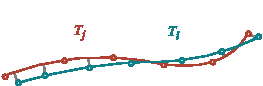
\includegraphics[scale=2.5]{trajectory-projection}
  \caption{An illustration of local distances from $\traj_2$ to
  $\traj_1$ as point-wise orthogonal projections.}\label{fig:trajectory-projection}
\end{figure}
This approach would eliminate the need to align observations before
comparing, however, it requires a continuous trajectory representation $h_{i}(t)$,
while observed trajectories are discrete samples. Assuming the samples
are jointly Normally distributed, and
come from a smoothly-varying function, a GP can be fit to the
observations to approximate $\obs_{i}^{(n)} = h_{i}(t)$. This GP will
model observations based on points in time, but the
\textit{exact points in time} are not relevant, since trajectories
for a single segment are generated at many different
occasions. Instead, consider modeling trajectory observations 
as $\obs_{i}^{n} = \modelf_{i}(\synchspace)$, where
$\synchspace = [0, 1]$ is the \textit{progress} from
start ($\synchspace = 0.0$) to finish ($\synchspace = 1.0$) of
a trajectory. This GP models observations based on
progression for any trajectory on a segment in a unified way. 
Finding a projection for point $\obs$ onto trajectory
$\traj_{i}$ can now be seen as finding how far along the trajectory $\obs$
would have traveled. More precisely, finding the $\tau$ that $\obs$
corresponds to. This can be done by fitting another GP to
$\tau = \synchf_{i}(\obs)$, which maps an observation onto the
progress relative to $\traj_{i}$. The projection onto $\traj_{i}$ is
then given by the composition $\synchedobs = (\modelf \cdot \synchf)(\obs)$.


as discrete samples. The samples can be seen as samples from a
smoothly-varying function of time $\obs_{i}^{(n)} = h_{i}(t)$, which
is naturally modeled by a GP.

$\traj_{i} = (\obs_{i}^{(1)},
\obs_{i}^{(2)}, \ldots, \obs_{i}^{(N)})$. 
Let $\traj_{i} = (\obs_{i}^{(1)}, \obs_{i}^{(2)}, \ldots, \obs_{i}^{(N)})$ denote trajectory
$i$ of length $N$, where each observation $\obs_{i}^{(n)} = (p_x, p_y,
v_x, v_y)$ contains position and velocity, and live in state space $\statespace$. 
A trajectory can be seen as a sequence of
samples from a time dependent, smoothly-varying function, which is naturally
modeled by a GP. In light of that observation, it is -reasonable to represent every observed trajectory as
a GP, and use the GP log likelihood to represent similarity. However
trajectories typically have different temporal lengths, which is
referred to as being \textit{unsynchronised}. To make comparisons in a
meaningful way, they need to have the \textit{same} temporal length,
that is, they need to be \textit{synchronised}. 
Figure~\ref{fig:unsynchronised-trajectories-fnames}, and
Figure~\ref{fig:synchronised-trajectories-fnames} illustrate the
concept of synchronised trajectories.
\begin{figure}
\begin{minipage}{.5\textwidth}
    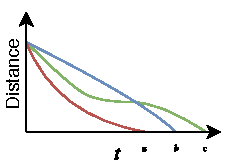
\includegraphics[scale=0.48,width=\textwidth]{unsynchronised-trajectories}
    \caption{Remaining distance for some route as a function of time for 
      unsynchronised trajectories. The functions cannot be
      fully compared, since the they have different support $[0, a]$,
      $[0, b]$, $[0, c]$.}\label{fig:unsynchronised-trajectories-fnames}
\end{minipage}
\hspace{5pt}
\begin{minipage}{.48\textwidth}
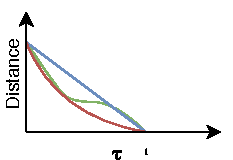
\includegraphics[scale=0.5,width=\textwidth]{synchronised-trajectories}
    \caption{Remaining distance for some route as a function of time for 
      synchronised trajectories. The motion patterns are comparable from
      start to end, since they all have support $[0, 1]$.}\label{fig:synchronised-trajectories-fnames}
\end{minipage}
\end{figure}

\subsection{Synchronisation Model}
Consider modeling observations from a trajectory as $\obs_{i}^{n} = \modelf_{i}(\synchspace)$ with an independent
multi-output GP for each dimension of $S$, where
$\synchspace = [0, 1]$ is the progress from
start ($\synchspace = 0.0$) to finish ($\synchspace = 1.0$) of
a trajectory. This model gives a way of to compare the
progression of $\traj_{i}$ with any other trajectory via the models likelihood, which for
a new observation $\newobs$ is
\begin{equation}
  \label{eq:model-log-likelihood}
  \begin{split}
    \log P(\synchspace|\newobs, {\modelf_{i}}) & = -\frac{1}{2}(\synchspace - \mu(\newobs)){[\Sigma]}^{-1}(\newobs - \mu(\synchspace)) \\
    & = -\frac{1}{2}\log{|\Sigma|}+C,
  \end{split}
\end{equation}
where $\mu(\newobs)$ and $\Sigma(\newobs)$ are given by
equations~\ref{eq:gp-mean-function},
and~\ref{eq:gp-covariance-function} for some $f_{i}$.
However, a way to compute $\synchspace$ for $\newobs$ is needed. This
is solved by using another GP to learn the inverse model $\synchf_{i} :
p\statespace \mapsto \synchspace$ for each trajectory $\traj_{i}$.
Any observation $\newobs$ can consequently be given a similarity metric
relative to $\traj_{i}$ by $\log P(\synchspace|\synchedobs,
{\modelf_{i}})$, where $\synchspace = \synchf(\newobs)$, and
$\synchedobs = (\modelf \circ \synchf)(\newobs)$.
\begin{figure}
  \centering
  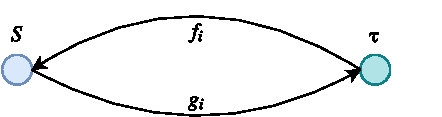
\includegraphics[scale=1.5]{synch-model}
  \caption{An illustration of the synchronisation model $\model_{synch}^{(i)}$, shown as 
    the mappings of $\modelf_i$ and $\synchf_i$. When synchronising a trajectory,
    it is mapped by $\modelf_i \circ \synchf_i$.}\label{fig:synch-model}
\end{figure}
Together, $\modelf_{i}$ and $\synchf_{i}$ make up the \textit{synchronisation
  model} $\model_{synch}^{(i)} = (\modelf_{i},  \synchf_{i})$ of $\traj_{i}$,
which is illustrated in Figure~\ref{fig:synch-model}.

\subsection{Learning the Synchronisation Model}
Learning a synchronisation model $\model_{synch}^{(i)}$ means learning
$\modelf_{i}$ and $\synchf_{i}$ by MAP estimation. However, there are
more constraints on the functions than can be formulated in
priors. In particular, a critical property of $\synchf_{i}$ 
is that it should be monotonically increasing in the direction of progression,
and stationary orthogonal to it. This is explained by the fact that a
vehicle is no closer to its destination should it drive more to the
left or right on a road; only the progression \textit{along} the road matters.
To enforce this property, data augmentation is used. 

When training GPs using a stationary kernel function, it is assumed
that the data is uniformly distributed, which is not the case for the
data available data set. In particular, during stand-stills, many
observations are generated in close proximity, which skews the
learning of the kernel lengthscale parameters to small values. To
avoid this problem, a technique called stop-compression is used.

\subsubsection{Data Augmentation}
\label{sec:data-augmentation}
For reasons previously described, $\synchf_{i}$ should be monotonically increasing in
the direction of progression and stationary orthogonal to it. 
To enforce learning such a function, each
observation $\traj_{i}^{(i)}$ is duplicated by placing a normal distribution
over it, orthogonal to the spatial progression vector ${(\traj^{(i+1)}_x -
  \traj^{(i)}_x, \traj^{(i+1)}_y - \traj^{(i)}_y)}^T$, and drawing several samples
with the same progression as $\traj^{(i)}$. This process is illustrated in
Figure~\ref{fig:traj-without-support-data} and
Figure~\ref{fig:traj-with-support-data}. 
\begin{figure}
  \begin{minipage}{.46\textwidth}
    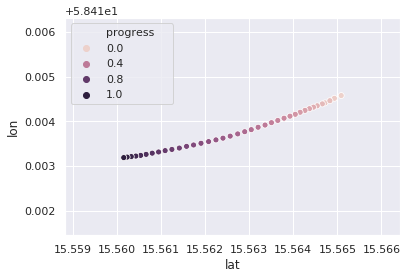
\includegraphics[scale=0.48,width=\textwidth]{traj-without-support-data2}
    \caption{Spatial progression of a trajectory 
      before data augmentation.}\label{fig:traj-without-support-data}
  \end{minipage}
  \hspace{5pt}
  \begin{minipage}{.46\textwidth}
    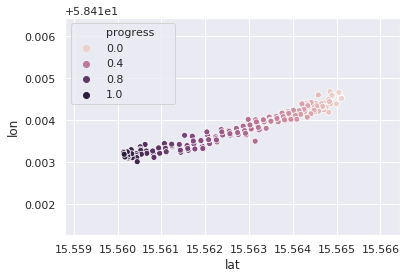
\includegraphics[scale=0.5,width=\textwidth]{traj-with-support-data2}
    \caption{Spatial progression of a trajectory 
      after data augmentation.}\label{fig:traj-with-support-data}
  \end{minipage}
\end{figure}

\subsubsection{Stop Compression}
\label{sec:stop-compression}
Stop compression aggregates observations in close proximity into a
single observation through averaging. Finding observations that should
be aggregated is done using... Kalman smoother talk to Tiger


\subsubsection{Similarity Metric}
A similarity metric can be defined by
\begin{equation}
  sim(\traj_{i}, \traj_{j}) = \frac{1}{M}\sum_{i=m}^{M}P(\traj_{i}^{m} | \traj_{i}),
\end{equation}
where trajectory $\traj_{j}$ has length $M$. The likelihood is
computed by synchronising $\traj_{j}$ using $\model_{synch}^{(i)}$. Observe that this metric is
not symmetric, nor does it satisfy the triangle inequality.
Consequently it is not a proper distance.

\subsection{Trajectory Clustering}
Clusters of one trajectory are currently considered.

\subsection{Arrival Time Prediction}
Why is this done from tau and not state?
\begin{figure}
  \centering
  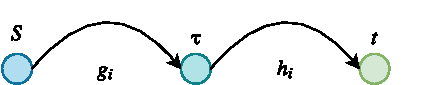
\includegraphics[scale=1.5]{prediction-model}
  \caption{An illustration of the prediction model. When predicting
    the arrival time for a trajectory, 
    it is mapped by $\predf_i \circ \synchf_i$.}\label{fig:synch-model}
\end{figure}